\documentstyle[11pt,psfig,subfigure]{article}

\def\papernumber #1 raised #2 {
\vspace{-#2}
\vbox to 0pt{\hfill\framebox{\bf Paper Number #1}}
\vspace{#2}
}

\title{Interactive TV}

\input epsf
% page layout
\addtolength{\topmargin}{-1in}    % move top margin up
\setlength{\textheight}{9.0in}      % text height
\addtolength{\oddsidemargin}{-0.5in}
\setlength{\textwidth}{6.25in}
\addtolength{\columnsep}{2.5ex}
%
%\setlength{\textheight}{6in}
%\setlength{\textwidth}{4.25in}
%
\addtolength{\itemsep}{-1ex}
%\addtolength{\topsep}{-1.5ex}
%\addtolength{\parskip}{2ex}

%space between lines-------
%default is 1
%\renewcommand{\baselinestretch}{1.3}    
\renewcommand{\baselinestretch}{1.0}    
%the value of \baselineskip is set by \bagin and each type-size-changing
%command to \normalbaselineskip * \baselinestretch.

%space between paragraphs ---------
%default is 0
\parskip=0.7\normalbaselineskip

%\newcommand{\versionLabel}[1]{ {\tiny #1} }


\newlength{\lineheight}
\setlength{\lineheight}{11pt}
\newcommand{\ls}[1]{\baselineskip=#1\lineheight}
\renewcommand{\baselinestretch}{1.0}
%\parskip = 0.7\normalbaselineskip
\parskip = 0.4\normalbaselineskip
\newcommand{\sspace}{\baselineskip=1.0\lineheight}
\newcommand{\nspace}{\baselineskip=1.2\lineheight}
\newcommand{\mspace}{\baselineskip=1.0\lineheight}
\newcommand{\aspace}{\baselineskip=1.0\lineheight}

\newenvironment{jlist}{
\begin{list}{$\bullet$}{
\setlength{\topsep}{0ex}
\setlength{\leftmargin}{1.5ex}
\setlength{\labelwidth}{1ex}
\setlength{\labelsep}{0.5ex}
\setlength{\itemsep}{0.6ex}
\setlength{\parsep}{0pt}
}}
{\end{list}}


\newenvironment{nlist}{
\begin{list}{}{
\setlength{\topsep}{0ex}
\setlength{\leftmargin}{1.5ex}
\setlength{\labelwidth}{1ex}
\setlength{\labelsep}{0.5ex}
\setlength{\itemsep}{0.6ex}
\setlength{\parsep}{0pt}
}}
{\end{list}}
                         
\author{Edward Y. Chang\\
Department of Electrical \& Computer Engineering\\
University of California, Sanata Barbara\\
echang@cs.stanford.edu}

\begin{document}
\date{}
%\maketitle

\mspace 
\newpage
\section*{PROJECT SUMMARY}
%\vspace{-.1in}

The goal of this research project is to build an infrastructure
that helps multimedia viewers interact with the content and 
change the pace of a televised program.
A fully interactive system (e.g., telepresence) would allow
the person to be immersed in a distant environment
and act upon it as if he was there, but we are far from
that capacity given the technology of the near future.
In this proposal, I present a receiver-based
architecture that supports {\em viewing interactivity}
and {\em content interactivity}. Viewing interactivity enables
a viewer to time-shift a televised program through
pause, fast-forward and instant replay operations. 
Content interactivity allows a viewer to query or to
change the content of multimedia data. 

With viewing interactivity, one can watch a program at 
whatever pace one finds comfortable. For instance, 
when one misses a crucial point while viewing a televised
lecture, one can replay the missed section and then 
continue viewing the lecture with a phase delay, or fast-forward
the lecture to get back in synch with the televised stream.
One can also record programs at multiple channels at the same
time, filter out unwanted
content and produce a customized program. 
(Using today's tape-based VCR, one cannot record
and replay a program or record more than one program 
at the same time.)
Content interactivity enables one to introduce one's 
creativity into a program.
For example, children would be able to change the attributes 
(e.g., colors, size, position and even the personality)
of the ``bunny'' and ``big bird'' 
characters in the {\it Sesame Street} program.  
With the capabilities to change both pace and content,
a class of high school students could conduct science experiments
in small groups through a virtual lab and their instructor
could keep track of their progress in real-time.   
Many other applications exist.

To enable viewing and content interactivity, 
we need a multimedia receiver that can display
more than one stream of TV, radio and the Web data,
can time-shift a stream, and can query and change
the content of a stream.  To accomplish these
goals, the multimedia receiver
needs a {\em buffer manager} that can schedule the
receiver's memory and 
disk bandwidth effectively to satisfy 
various interactive scenarios, and it needs a {\em data manager}
that can manage data from TV, radio and the Web 
for supporting efficient queries and retrieval.

Although progress has been made in buffer and
data management, many issues, especially in managing multimedia
data and managing buffer for rendering and
for querying multimedia data,
and in developing an architecture that can be adaptive
to both resource constraints and {\em Quality of
Service} (QoS) requirements, remain open.
I plan to address these issues, and to build on
work from several fields, most notably from the
image processing, operating system and database fields.
In particular, I am interested in developing the 
following technologies:

\begin{nlist}
\item {\bf 1}.
Temporal indexing structures that support
efficient stream synchronization.
\item {\bf 2}. Caching and prefetching techniques that satisfy
the real-time data requirement of the continuous media data
(i.e., video and audio) on the one hand, and minimize the
initial latency in responding to an interactive request
on the other.
\item {\bf 3}.  
QoS-adaptive buffer-management architectures that manage
memory and disk bandwidth by adapting to
the receiver's resource constraints and
the viewer's QoS requirements.
\item {\bf 4}.
Media query processing that handles heterogeneous
media queries efficiently. 
\end{nlist}

In addition, I envision constructing demonstrations 
that use these technologies.
Here is a list of some of the demonstrations I am planning
to indicate the progress of this project:
\begin{jlist}
\item 
A multimedia database that supports content-based 
queries,
\item 
A digital VCR that supports pause, fast-forward and instant 
replay, and
\item 
A multi-camera video surveillance system (e.g., for 
monitoring in a nuclear power facility).
\end{jlist}

%The multimedia database system provides the digital-VCR 
%project with an efficient storage and an effective query 
%engine that can help the viewer select content 
%before the viewer issues a fast-forward or replay command.
%The digital-VCR, which receives only one stream at a time,
%in turn, is extended by the multi-camera video surveillance project,
%which handles multiple cameras, streams and viewers simultaneously.

Finally, my education objectives include the expansion of
the curriculum in database and multimedia systems at U.C. Santa
Barbara. In particular, a new course that I am developing
will cover the latest 
trends in database and multimedia systems. 

In summary, this project will develop an infrastructure 
that provides a framework for building
a wide variety of interactive multimedia applications
in the educational, commercial, government and
military sector.


\nspace 
\newpage
%\section{RESEARCH PLAN}
\subsection{Motivation}

Traditionally, watching a television program has been a passive experience:
All viewers receive the same TV content at the same
playback pace, regardless of individual preferences.
Not being able to select viewing pace 
can be inconvenient and even unproductive 
sometimes. For instance, when one
is interrupted while watching a news program
(say, by a phone call or biological need), one may 
miss the information (e.g., stock quotes, weather forecast,
etc.) that one has been waiting for.  Similarly, when
one misses a crucial point while viewing a televised
lecture, one may not be able to comprehend the materials
after that point.
What is desirable is {\em viewing interactivity}
---pause, fast-forward and instant replay---allowing
the time-shifting of a program so the viewer can
watch at whatever pace he or she finds comfortable.
One can also record programs at multiple channels at the same
time (which a tape-based VCR cannot do), filter out unwanted
content and produce a customized program. 

In addition to viewing interactivity, being able to 
interact with the content of a program (what I call
{\em content interactivity}) can enrich viewing experience.
Content interactivity is
especially beneficial for educational programs. For instance,
children would be able to change the attributes 
(e.g., colors, size, position 
and even the personality) of the ``bunny,'' ``big bird'' and
other characters in the {\it Sesame Street} program.
A grade school student can learn American states
by interacting with a map.
A class of high school students could conduct science experiments
in small groups through a virtual lab and their instructor
could keep track of their progress in real-time. 
Many other applications exist.

To support interactivity, many studies suggest a server-based
architecture (e.g., \cite{ex80,ex49,ex54,ex1,ex86}),
in which a server schedules
its resources (i.e., memory and disk bandwidth)
to support interactivity.
In a server-based architecture, the receivers are assumed
to be passive---simply receiving bits and rendering frames.
However, because of the typical long end-to-end transmission
delay between a server and a receiver and the Interet's limited bandwidth,
it is practically infeasible for the server
to support ``real-time'' viewing interactivity for tens of
thousands of simultaneous users.  Furthermore,
on a broadcast channel (e.g., CNN), one simply cannot request
the server to pause or replay a program.
 
Instead of the server-based approach, I plan to investigate
new hybrids of technologies for 
a receiver-based architecture to support viewing interactivity 
and content interactivity. Figure~\ref{fig-dtv-pipeline} depicts a 
multimedia data delivery pipeline.  A receiver in this architecture
is equipped with a large and inexpensive disk and may have an 
Internet back-channel in addition to the broadcast channel.
The economical caching together with the random
access capability of the disk enables a multimedia receiver to 
buffer a large amount of data to support
time-shift operations.  A viewer can pause a live 
program to take a break from viewing while the broadcast
stream continues arriving and being written to the local disk.
The viewer can resume watching the program after the pause
with a delay, or fast-forward the program to get back in synch with
the broadcast stream.  
While a given broadcast stream remains the same
for all viewers, various data objects can be transmitted to
individual viewers via the Internal channel.
Image-based rendering techniques can
overlay a number of data objects with the broadcast stream to
produce a customized program for content
interaction.

\begin{figure}[t]
\epsfxsize=350pt
\centerline{\epsffile{fig-dtv-pipeline.eps}}
\caption{The Multimedia Data Delivery Pipeline.}
\label{fig-dtv-pipeline}
\vspace{.1in}
\end{figure}

Extending the DRAM cache with a large disk and
adding an Internet channel to the receiver add complexity to 
the receiver's buffer and data management. To ensure that IO 
are efficiently scheduled, the receiver needs a 
{\em buffer manager} that can schedule the
receiver's memory and
disk bandwidth effectively to service
a wide variety of interactive scenarios.
The receiver also needs a {\em data manager}
that can manage data from TV, radio and the Web
for supporting efficient queries and data
retrieval. Although progress has been made in these areas,
many issues, especially in managing multimedia
data and managing buffer for rendering and
for querying multimedia data,
and in developing an architecture that can be adaptive
to both resource constraints and {\em Quality of
Service} (QoS) requirements, remain open.
(These challenges are discussed
in detail in Section~\ref{sec-challenges}.)
I plan to address these issues, and to build on
work from several fields, most notably from the
image processing, operating system and database fields.
In particular, I am interested in developing the
following technologies:
                             
\begin{nlist}
\item {\bf 1}.
Temporal indexing structures that support
efficient stream synchronization.
\item {\bf 2}. Caching and prefetching techniques that satisfy
the real-time data requirement of the continuous media data
(i.e., video and audio), on the one hand, and minimize the
initial latency in responding to an interactive request,
on the other.
\item {\bf 3}.
QoS-adaptive buffer-management architectures that manage
memory and disk bandwidth adaptively to
the receiver's resource constraints and
the viewer's QoS requirements.
\item {\bf 4}.
Media query processing that handles heterogeneous
media queries efficiently.
\end{nlist}   

In addition, I envision constructing demonstrations
that use these technologies.
Here is a list of some of the demonstrations I am planning
to implement:
\begin{jlist}
\item 
A multimedia database that supports content-based
queries,
\item 
A digital VCR that supports pause, fast-forward and instant
replay, and
\item 
A multi-camera video surveillance system (e.g., for
monitoring in a nuclear power facility).
\end{jlist}

The multimedia database system provides the digital-VCR
project with an efficient storage and an effective query
engine that can help the viewer select content
before the viewer issues a fast-forward or replay command.
The digital VCR, which receives only one stream at a time,
in turn, is extended by the multi-camera video surveillance project,
which handles multiple cameras, streams and viewers simultaneously.
These demonstrations show that 
a wide variety of interactive multimedia applications
in education, commercial, government and
military sectors can be built on the technologies
developed in this project.
                           
Much of the research I propose will be joint efforts
with colleagues and students at the University of California,
Santa Barbara and Stanford University.

In the remaining sections of this proposal, I enumerate the challenges
this project faces, the core technologies I plan to develop, 
my prior accomplishments, and
the demonstrations I plan to implement.   

\subsection{Technical Challenges}
\label{sec-challenges}

A multimedia receiver faces at least three design challenges:
\begin{jlist}
\item Not all data are equal: different types of data may have different
size and latency characteristics.
\item Not all receivers are equal: different receivers may have different
available hardware resources and network bandwidth.
\item Not all viewers are equal: different viewers may have different
viewing preferences.
\end{jlist}
In the remainder of this section, I enumerate these challenges.

\subsubsection{Not All Data Are Equal}

\begin{figure}[t]
\epsfxsize=260pt
\epsfysize=160pt
\centerline{\epsffile{fig-dtv-data.eps}}
\caption{The Characteristics of Multimedia Data Objects.}
\label{fig-dtv-data}
\end{figure}

Multimedia data objects can be continuous, textual, binary,
and so forth.  These data objects are
best characterized by their {\it sizes}
and {\it latency constraints}. Continuous       
data are audio/video streams, which are voluminous and
delay sensitive.
Textual data include captions, HTML and XML documents,
etc. Textual data occupy far less space than continuous data
and are not as delay sensitive. Other data, such as images and applets,
can be very copious or scant and may or may not be delay sensitive,
depending on the nature of the application.
Figure~\ref{fig-dtv-data} shows the characteristics of
these data objects. The $x$-axis in the figure represents the
delay sensitivity from low (on the left-hand side) to high
(on the right-hand side); the $y$-axis gives the size of an object.
At one extreme, videos are large and very sensitive to
delay. At the other extreme, captions are small in size and not very
sensitive to delay.
                       
\begin{figure}[t]
\epsfysize=160pt
\epsfxsize=280pt
\centerline{\epsffile{fig-delay-fs.eps}}
\caption{Delay Functions.}
\label{fig-delay-fs}
\end{figure}

When allocating memory and disk bandwidth for data objects, both 
their sizes and latency constraints must be taken into consideration.
We plan to characterize each data object's size and latency 
characteristic as follows:
The size of a data object is measured by the 
amount of storage space it needs.
The delay sensitivity of a data object is quantified as
a value function.  
As Figure~\ref{fig-delay-fs} shows, 
the function can be defined in many ways
(the $x$-axis in the figure depicts delay; the $y$-axis
depicts the value of the object normalized to
from zero i.e., worthless, to one): Function $F_a$
depicts an object that can tolerate delay up to a period $t_\delta$.
Function $F_b$ shows the value of an object that decays linearly
after $t_\delta$. Functions $F_c$ and $F_d$ have other
value decay patterns.                                 
In terms of data streams,
function $F_a$ is a good value function for an audio frame,
function $F_b$ may be a good value function for a video
frame since slight delay of a frame display may be tolerable,
function $F_c$ may be a good value function for a subtitle, and
function $F_d$ may be a good value function for a Web page.
                                                       
\subsubsection{Not All Receivers Are Equal}

The critical resources of a receiver include memory,
network bandwidth and disk bandwidth.
These resources can also be characteristized by their
capacity and latency. The memory
size and the disk size
are both constants that
can be obtained from the system configuration file.
The latency of a receiver
is best characteristized by the IO time between memory
and the local disk since this latency dominates the latency
in the storage hierarchy. The IO time for reading/writing
data object $i$ (denoted as $\tau_i$) can be written as:
$\tau_i = \gamma(d) + S_i/TR$,
where $\gamma(d)$ is the seek time and rotational
delay of the disk given $d$ tracks to seek before transferring
data, $S_i$ is the size of the $i^{th}$
data object, and $TR$ is the transfer rate of the disk.
Note that the latency just described
assumes that no IO conflict exists. In reality, the          
more objects are accessed, the longer the delay that
can be experienced by an IO.  
Scheduling conflicts must be taken
into consideration and must be resolved
in an order that achieves maximum total QoS
for the viewer.
                                             
\subsubsection{Not All Viewers Are Equal}

To measure a viewer's satisfaction, we must allow the
user to have a say about what is important and
what is not. We thus associate each data object
with a QoS parameter. A viewer can
assign a QoS value to each data object, either
implicitly or explicitly.
For instance, if a user decides to turn off
all interactive features, the resource manager can
assign a QoS factor of zero to data objects
that are needed to support interactive features.
Regarding the data objects that are
needed to support the playback, higher QoS can be assigned to
mission-critical data objects, such as broadcast
video and audio streams and lower QoS can be assigned
to optional data objects such as captions and applets.


%\section{Core Technologies}
\label{sec-core}

In the following paragraphs, I enumerate the technologies
we plan to work on to tackle the challenges, 
beginning with our efforts in synchronizing media streams.

\subsection{Temporal Indexing for Scene Synchronization}

Content interactivity allows a viewer to change the content
of a program locally. For instance, the viewer can change
the attributes (e.g., colors, positions and speed)
of the objects in a scene. 
Content interactivity can be enriched if the TV is connected
to a bi-directional Internet back-channel.
Using distance education as an example,
a student can interact with a 3D globe
during a world geography lecture.
The instructor can quiz the students on-line to understand 
how the students absorb the lecture materials and can make real-time
adjustments.

To support content interactivity, the receiver must synchronize
the rendering of the data objects in a scene. 
%Fortunately, much low-hanging fruit 
%in this area is ready to be plunked. 
This knowledge is already available.
For example, MPEG-4 \cite{Mp4} has proposed standards to
separate interactive objects from the scenes, to change
visual or acoustic properties of an object, and to
specify the spatio-temporal relations between objects.
Many studies have also proposed synchronization models
and languages \cite{Hyp92,Co96,Gr95,Ha96,HFK95,Hkm97}.
However, neither MPEG-4 nor these studies 
address {\em data organization}
and {\em QoS adaptivity} issues, issues I intend to investigate.

\begin{figure}[t]
\epsfysize=140pt
\centerline{\epsffile{fig-scene-desc.eps}}
\caption{An Example Scene Description.}
\label{fig-scene-desc}
\end{figure}
                  
Figure~\ref{fig-scene-desc} shows a schematic example of these issues,
an MPEG-4 scene description of a simplified geography
lecture. The scene at its top level is divided into four
objects: a 2D background, furniture, a white board and 
an instructor.
The furniture ``object'' consists of a desk, a chair and a globe
``subobject.''  The instructor object consists of a 
voice and a sprite subobject.  
Of these objects, a student 
can interact with the white board and the globe.
What this means is that the 2D background and the instructor 
are broadcast via satellite, and the furniture and white board
are delivered via the Internet. The receiver faces the
challenge of synchronizing
these two streams in both spatial and temporal dimensions.

To simplify our discussion,
let us focus on the temporal synchronization.
The receiver must properly synchronize two streams in the temporal
dimension.  If streams are delivered and
rendered in real-time, the temporal synchronization may not be
a major problem since the receiver can render the objects in
the streams as they arrive. However, if the viewer issues a 
pause, the streams may be stored on the local disk, and how 
they are stored on disk will affect their subsequent
retrieval. 
%For example, the 
%temporarily related objects can be stored contiguously
%on disk. This approach, however, may not be feasible
%if objects appear in many scenes.
%Various data organization policies will be experimented with
%to discover rules for storing temporally related data.

When a data object
is referenced, it and all its temporally related objects should be
found quickly, and, once requested, be retrieved efficiently.
Indexing temporally related objects can be tricky.
In principle, all temporally related object should be
stored contiguously on disk to minimize the disk latency
necessary to retrieve them.
However, since an object may be shared in many scenes,
replication may not always be desirable. One alternative is
storing shared objects in the middle tracks so their
access latency is constrainted. Another alternative
is storing shared objects on the outer tracks to take
advantage of their higher data transfer rates.
We will experiment with various data placement policies to
examine if some rules of thumb can work most of the time.

It seems that building temporal indexes at the scene level is
appropriate. Once a scene can be located, the
scene description can tell where its data objects
reside. I believe that the combination of hashing and XML
may be an appropriate structure for indexing scenes \cite{PBC99}.
A hash table provides fast scene lookup; XML
provides the flexibility to describe semistructured
objects in a scene. We will investigate how to
deal with efficient updates (primarily necessary because of changes
of the object's location)
and queries on XML structures \cite{Abi97,Bun97,MW99}.

One useful feature that the receiver can support is video
editing (changing the temporal sequence of 
scenes). A video editing tool can combine scenes from
different videos into a customized clip. Supporting
video editing introduces additional scene management issues.
When a scene is shared by two or more clips, the scene
should not be copied entirely. A scene is copied only
when its substantial content is modified. Otherwise,
we may want to create a shell scene, which maintains
links to its parent scene and keeps only those objects that it
modified.
              
\subsection{Caching and Prefetching Techniques}

Viewing interactivity allows viewers to select their own
temporal view of the TV content in real time.
A temporal view is created by a time-shift VCR-like 
operation---pause, replay or fast-forward. Extending a DRAM cache
by adding a disk increases the cache size and thereby
enables the support of these time-shift operations economically.
However, adding a disk to a DRAM cache also increases the complexity of
the receiver's buffer management.
This increased complexity is primarily introduced by the fact that
video and audio data must be made available continuously
to meet {\em real-time} playback deadlines \cite{ex9}, or playback 
interruptions occur. In addition, to achieve acceptable 
interactive performance,
the buffer manager must make the requested data available
in main memory with {\em minimum initial latency}, e.g.,
when a viewer issues a replay, the response time should be very short.
Satisfying these two potentially conflicting performance 
objectives with minimum DRAM (and hence at minimum cost) 
is a challenging design task.
For instance, in the geography lecture example, a
student my click on the globe object on the desk to request a
video clip about the earth, while the instructor
is speaking. We do not want to interrupt the
continuation of the audio track but we also want
to render the video clip as soon as possible.
To deal with these conflicting goals will be a challenge.

Much work has been done at the server side to schedule IOs
for retrieving
multimedia data \cite{ex121,ex86,ex8-1,ex18,ex302,ex10}.
It is important to note that the {\em receiver-side}
analysis differs from these more
``traditional'' server-side analyses.
In particular, in a server environment, the server has full control of
the data generation rate, while at the receiver, data arrival (from
the network) is unpredictable.
In other words, the server schedules events while the receiver
reacts to events.

To achieve minimum initial latency,
the buffer manager
must be able to service an interactive request
promptly. Since the disk IO is the bottleneck of
the performance, the objective is to schedule IOs
in the right order so that the disk arm on the one hand can
quickly service the newly requested
interactive task and on the other hand can fulfill
the real-time constraints of other data objects.
                                         
Three techniques for making IO scheduling more flexible can
be explored. They are: {\em data
prefetching}, {\em caching}, and {\em data placement}.
When the disk bandwidth is under-utilized, the disk
can be scheduled to perform prefetching
for continuous data so that when
an interactive request arrives, a sufficient amount of
continuous data has
been staged in main memory to meet their real-time
requirements. This gives the disk arm
freedom to service the interactive request immediately.
To minimize the DRAM requirement (and hence reduce the
cost of the receiver), the buffer manager
should minimize disk latency, which requires implementing
intelligent disk-scheduling and data-placement policies.
We will evaluate the tradeoffs between
various factors (e.g., cost, speed and complexity) and devise
efficient and cost-effective buffer management strategies
for the receiver to meet the low initial latency goal 
under real-time data constraints.
                              
\subsection{QoS-Adaptive Buffer Management}

Adding complexity to the problems, the buffer manager must be
{\em QoS adaptive} and must be able to scale gracefully in the following
two areas:
\begin{itemize}
\item Resources:
As mentioned earlier, the
available hardware resources can differ from one receiver
to another. The local resources may not be adequate
to support a particular interactive scenario.
For instance, interacting with an object in a scene 
may require downloading a high
resolution video clip, which the processor cannot decode
in real-time.  Therefore, it is critical for the resource 
manager to be adaptive to
the resource constraints and to degrade, if degradation is
unavoidable, in a graceful manner.  
\item QoS requirements:
The QoS preference can be different from one viewer to another.
For instance, some students watching a televised lecture 
may prefer seeing the write board
to the fidelity of the video, or vice versa.
\end{itemize}

The degradation of content can happen on two different
levels: on the object level and on the scene level.
                                                 
\begin{itemize}
\item On the object level, a layered coding scheme can
be used so that only selected layers are decoded to achieve
the targeted QoS.  Much effort has been devoted to developing a
layered coding scheme that supports scalable QoS \cite{ex220,ex62},
and there have also been studies on QoS adaptivity
in the network transport layer \cite{ex56,ex96,ex95}.
We will evaluate these technologies and choose the ones
that suit our needs.

\item On the scene level, some data objects
that are occluded can be kept from
being processed. The remaining objects can be scheduled
based on a combination of the viewer's QoS specification
and the delay functions of the data objects. The goal
of the scheduler is to maximize the total QoS
under the resource constraints.
Suppose that in the geography lecture example the
system resources cannot render both the white board object
and the instructor object. In this case the resource manager
renders the object that receives a higher QoS assignment   
from the student.
\end{itemize}

The challenge posed by all the above issues---caching, data prefetching
and placement, QoS-adaptivity, initial latency, real-time
data constraints and cost---will be to
devise a resource management policy that satisfies all
requirements at the same time.
To achieve this aim, we plan to
first develop effective techniques for caching, data
prefetching and placement, and scheduling, and then to
combine individual techniques to achieve our global
objective: maximizing QoS. We plan to
formulate the resource management plans quantitatively.
Our preliminary idea is to develop a model that considers all
constraints together with QoS requirements
and that can be solved efficiently in real time
for a schedule that achieves maximum total QoS.
                                                     
\subsection{Media Query Processing}

To support effective time-shift operations, the receiver needs
a {\em search engine} that supports fast lookup and retrieval
of the viewer's desired video clip. For instance, a
viewer may want to replay a particular section of a
lecture in which the history of television is discussed.
The search engine looks up the indexes to find
scene descriptors that best match the key words ``television
history'' and returns
a list of scenes in a ranking order.
Another way to specify a query is content-based. The viewer can draw
an object and its trajectory \cite{Ccmsz97}, and 
the search engine finds
and returns the scenes that have a similar object 
moving in the same trajectory. 

For each video, the search engine builds its scene descriptors and stores
these descriptors in the database.  This process can be divided into
two major steps: {\em feature selection} and {\em indexing}. 

{\it Feature selection}
has enjoyed much attention lately, as is witnessed by the
large number of recent articles on it.
For example, \cite{Ccmsz97,Hjw95,Mmz95,Mc96,Zks93} propose
feature extraction techniques for video, \cite{Bc94,Pfe96} for audio
and \cite{img11,img12,img13,Pps96,Pzm96,Hkm97} for images.
In addition to evaluating and using some of these
existing approaches, we will experiment with 
a {\em variance control model}
that decides how fine the features used should be 
based on 1) the user's definition of a ``match'' 
and 2) the size of the database.  Take image searching as an example.
If one wants to find near-copies of an image,
the search engine should extract fine details
from the query image and perform a close match.
If one wants to find  
images of similar colors that are not necessarily
at the same spots, the seach engine
can extract a coarser color distribution from the query image
to perform the lookup.  Consider the
size of the database. While a small database 
(the typical database of a receiver) requires a 
small set of features to tell media objects apart, a
large image database (the typical database of a content provider)
requires a large set of features.
Intuition tells us that the selection of features
during the indexing and query processing steps
should depend on the semantics of
the search, the size of the database, and the 
available resources.  We will investigate
if this variance-controlled approach can be fruitful.

Content-based retrieval
is inherently expensive, especially when
it needs a large number of dimensions to characterize the
target object (e.g., an image or a video scene).
There is simply no way to
build an index on disk such that {\em all} nearest neighbors to {\em
any} query point are physically near on disk.
Fortunately, in many cases it is
sufficient to perform an {\em approximate search} that returns many
but not all nearest neighbors~\cite{AM94,Cla94,IM98,Jk97,KOR98}.  (A
feature vector is often an approximate characterization of an object,
so we are already dealing with approximations anyway.)
I have recently proposed a
clustering/indexing combined scheme that achieves approximate
similarity search with high efficiency \cite{Lch99}.
This proposed clustering/indexing combined scheme should
provide a solid foundation for continued work,
but many challenges remain. We are, for one, not
convinced that the Euclidean distance
is the only way to measure similarity for multimedia data.
Thus, we are investigating other similarity measures
(e.g., Hamming distance, etc.). For another,
we think similarity should be personalizable.
We will thus investigate new measures for similarity.

Finally, a challenging issue about building indexes for video scenes
is that some scenes may have missing features and that different
scenes may be best represented by different sets of
features.  For instance, the video frames in a lecture and in a news program
may provide little useful information about the content
of the program if all they show is a ``talking head.''
In this case, using their audio tracks
and text captions may better tell the content. For scenes that
have motion, on the other hand, audio tracks and captions may not be useful.
Rather, the motion vectors in the inter-coded frames
can tell the speed and trajectory
of the moving object. We plan to investigate if
assigning different weights to different features may 
help promote those features with greater significance.
We will also investigate techniques that can deal
with missing features when indexes are built.



%\section{Core Technologies}

In addition to investigating new techniques for managing
system resources and data, we will attempt to share a common image
representation for both resource and data management.
Traditionally, the image processing community and the database 
community have been developing their own image representations, i.e.,
the image processing community proposes 
compression algorithms and the database community proposes image
feature representations (e.g., color histograms).
A fascinating research direction may be to build search indexes 
on the compressed data directly. We are especially interested
in exploring {\em layered coding} techniques that can support
both scalable content degradation and scalable content-based indexing.

Finally, our design goal is not only to provide the 
interactive functions, but also
provide these functions with minimum resource requirement
(hence at minimum cost) and with minimum initial latency.
In the following sections, I enumerate the technologies 
we plan to work on, beginning with our efforts in resource
management. 

\subsubsection{Indexing for Temporally Related Data}

When a data object
is referenced, it and all its temporally related objects should be
found quickly, and once requested, be retrieved efficiently. 
Indexing temporally related objects can be tricky.
In principle, all temporally related object should be 
stored contiguously on disk to minimize the disk latency 
necessary to retrieve them.
However, since an object is often shared in many scenes,
replication may not always be desirable. One alternative is
storing shared objects in the middle tracks so their
access latency is constrainted. Another alternative
is storing shared objects on the outer tracks to take
advantage of their higher data transfer rates. 
We will experiment with various data placement policies to
examine if some rules of thumb can work most of the time.

It seems that building indexes at the scene level is
appropriate since a scene is a reasonable search 
unit (why this is so is discussed further 
in the content-based retrieval section,
which follows). Once a scene can be located, the 
scene description can tell where its data objects
reside. I believe that the combination of hashing and XML
may be an appropriate structure for indexing scenes.
A hash table provides fast scene lookup; XML
provides the flexibility to describe semistructured
objects in a scene. We will investigate how to
deal with efficient updates (primarily necessary because of changes
of the object's location)
and queries on XML structures \cite{Abi97,Bun97,MW99}.
Another challenging problem and a new research direction
is performing similarity queries on semi-structured 
data that is in XML format.

One useful feature that the receiver can support is video
editing. A video editing tool can combine scenes from
different videos into a customized clip. Supporting
video editing introduces additional scene management issues.
When a scene is shared by more than one clip, the scene
should not be copied entirely. A scene is copied only 
when its substantial content is modified. Otherwise,
we may want to create a shell scene, which maintains
links to its parent scene and keeps only those objects that it
modified. 

\subsubsection{Indexing for Content-Based Retrieval}

To support effective time-shift operations and general
multimedia database queries, we
intent to build a content-based video scene
retrieval system. 
A video can be divided into a number of sequences,
a sequence a number of scenes, and a scene a number
of frames.  We believe that a scene should be a reasonable
query unit. Supporting queries on the frame level 
is simply too expensive (a one-hour video
at 25 frames/second frame rate has $90$K frames).
Furthermore, indexing on the frame level 
cannot describe motion, e.g., a bus is approaching.
Supporting queries on the sequence level
may be too coarse and may hurt query precision.
Therefore, we plan to build scene descriptors
and build indexes on these scene descriptors.

Building such a system faces
four challenging steps: 1) selecting and extracting features from
multimedia data objects, 2) clustering the extracted features,
3) indexing objects based on their feature clusters, and 4) devising
query processing steps that find matches efficiently
in the database.

Selecting and extracting features can be complicated.
Fortunately, much low-hanging fruit in this area is ready to be plucked.
We plan to rely
on existing tools as much as possible. For feature clustering,
a large number of papers \cite{img11,img12,img13}
have been published with many of
ideas. Instead of coming up with yet another feature
cluster, we will experiment with a variance control model
that will decide how fine the features must be clusters to attain
good similarity results.
Take image searching as an example.
If one wants to find near-copies of an image,
the feature cluster should record finer details 
of the color distribution on the query image. If one wants to find
images of similar colors that are not necessarily
at the same spots, the feature vector can record 
coarser color distribution. 
Extensive exploration and experiments will 
be performed to verify if this variance controlled 
approach can be fruitful.

Content-based retrieval 
is inherently expensive, especially when
it needs a large number of dimensions to characterize the
target object (e.g., an image or a video scene).  
There is simply no way to
build an index on disk such that {\em all} nearest neighbors to {\em
any} query point are physically near on disk.  
Fortunately, in many cases it is
sufficient to perform an {\em approximate search} that returns many
but not all nearest neighbors~\cite{AM94,Cla94,IM98,Jk97,KOR98}.  (A
feature vector is often an approximate characterization of an object,
so we are already dealing with approximations anyway.)  
I have recently proposed a
clustering/indexing combined scheme that achieves approximate
similarity search with high efficiency \cite{Lch99}.
This proposed clustering/indexing combined scheme should
provide a solid foundation for continued work,
but many challenges remain. We are, for one, not
convinced that the Euclidean distance
is the only way to measure similarity for multimedia data.
Thus, we are investigating other similarity measures
(e.g., Hamming distance, etc.). For another,
we think similarity should be personalizable.
We will thus investigate new measures for similarity.

Finally, 
for query processing, we will investigate 
data models, query languages and query optimization techniques.

%\subsection{Image Coding and Packetization}
%\label{sec-image}
%
%The researchers in the compression
%camp have been devised compression techniques 
%for coding efficiency and robustness. The
%researchers in the database camp have been devised
%indexing data organization schemes for efficient data retrieval.
%Researchers in two camps often characterize an image 
%differently. Consequently, an image may have one
%representation (e.g., JPEG) in transmission and
%another representation (e.g., color histograms)
%for the indexing phase. 
%It would be nice if two efforts can
%share one common data representation. At this time, wavelets
%seem to be an attractive choice.
%Wavelets' scalability fits well
%for supporting both scalable content degradation and
%scalable content-based indexing.
%
%%While studying image representation, we also want to
%investigate how an image should be packetized to
%be more error resilient.
%One idea is that for the base image/audio/video layer, 
%forward error correction (FEC) code can be applied to
%improve its error resiliency. For progressive layers, 
%however, we may not want to
%spend additional bits on channel encoding. Instead, we can rely on 
%error concealment and reconstruction techniques to
%recover an image after encountering channel errors.
%
%We will also investigate image-based rendering techniques.
%At this end, our focus is on video panoramas for supporting
%spatial viewing interactivity.
%For a single camera, supporting
%video panoramas requires a method for locating
%frames that contain smooth
%camera pans or tilts, from which the panoramic
%view can be synthesized.
%

%\subsection{Putting All the Pieces Together}



%\subsection{Put All the Pieces Together --- Demonstration Plan}

We plan to build three systems to demonstrate our research
results: A content-based video scene retrieval system, a digital VCR
that supports both viewing and content interactivity, and
a multi-camera video surveillance system. 
The content-based scene retrieval system
provides the digital-VCR project with an
efficient storage and an effective query engine that can help
the viewer select content
before the viewer issues a fast-forward or replay command.
The digital VCR, which receives only
one stream at a time, in turn, is extended
by the multi-camera video surveillance project, which 
handles multiple cameras, streams and viewers simultaneously.

\subsubsection{A Content-based Video Scene Retrieval System}

The content-based search engine receives a query 
from a user. The query can consist of an image/drawing and 
some key words. The search engine profiles
the image/drawing, together with the specified
key words, and it finds the matching scenes in its repository
and returns them to the viewer in a ranking order.   
The key technologies demonstrated via this prototype are
1) the search engine's feature clustering and
indexing can scale well with respect to
the receiver's available resources and the size of
the database, and 2) the search engine can index 
features with different importance and can
cope with missing features.
%We will show that queries such as
%``Find all scenes in which a man is walking by a car''
%can be retrieved effectively.

{\bf Core technologies demonstrated}: 
feature clustering, indexing and query processing.

\subsubsection{A Digital VCR}

\begin{figure}[t]
\centerline{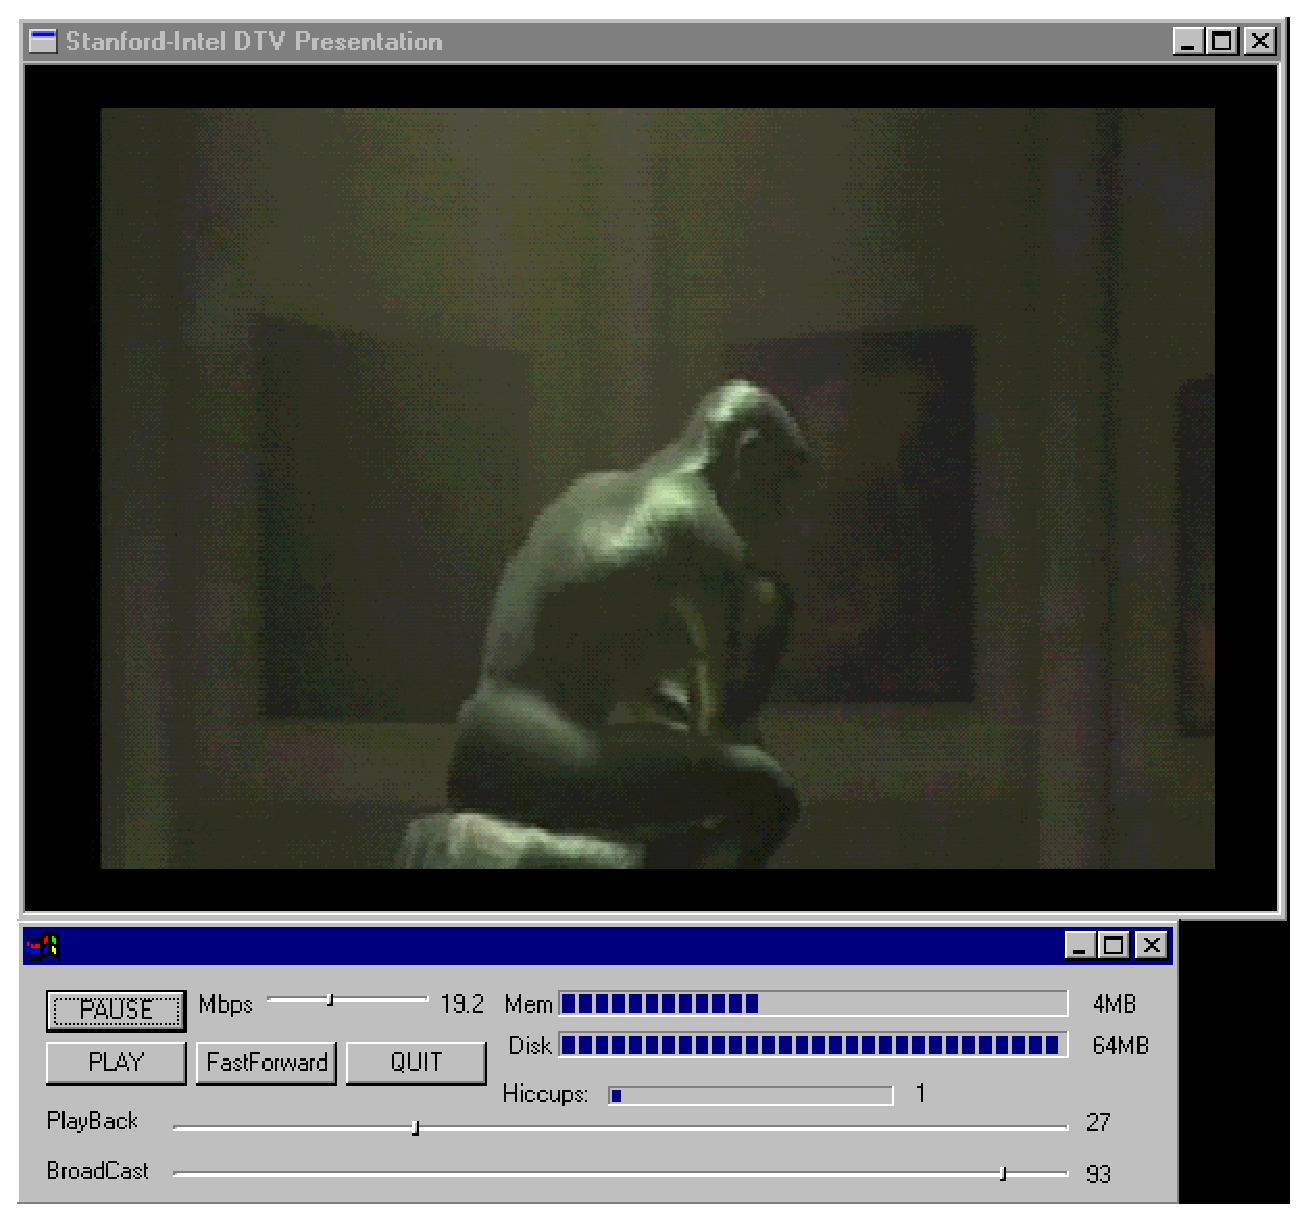
\psfig{figure=digital_vcr.ps,width=300pt,height=200pt}}
\caption{A Digital VCR Screen Shot.}
\label{fig-codec}
\end{figure}

The implementation of a
Digital VCR that supports VCR-like interactive functions including
{\em pause}, {\em fast-forward} and {\em instant replay} is under way.
Figure~\ref{fig-codec} shows a screen shot of the user interface
(i.e., {\em codec}) and display.
At the bottom of the figure is the codec through which a viewer
issues interactive commands and monitors the system.
To issue a command, a viewer selects and presses one
of the control buttons on the upper-left corner of
the codec (described shortly). To help visualize
the system, the codec uses trackbars to display various statuses. The five
trackbars from the top to the bottom on the codec keep track
of the amount of memory use, the amount of disk use,
the accumulated number of hiccups, the playback progress,
and the broadcast progress. 
In the final phase of this project we
will incorporate the content-based video scene search engine
into the digital VCR for supporting scene
queries before the viewer issues a fast-forward or replay request. 
                          
%When a viewer watches a TV program live, memory is
%used to buffer the mismatch between the data transmission
%rate and the playback rate. The memory trackbar keeps
%track of the current memory use. The disk use
%is zero when a program is watched live. When the pause button
%is pressed, the excessive data that the DRAM cannot stage is
%written onto the disk. Using the disk as a part of the
%cache, the VCR can allow the viewer to pause for a substantial amount
%of time (a $9.1$ GBytes disk can buffer more than one hour of
%$19.2$ Mbps DTV program).  After returning from the break, the viewer
%can press the {\em play} button to resume the playback. At
%this time, the decoder consumes data from the disk while the
%broadcast data continue arriving and being appended to
%the tail of the disk file. The viewer has the option to
%perform {\em fast-forward} to catch up with the live
%program. When the fast-forward button is pressed, the Digital VCR
%retrieves data from the disk at a faster pace and the decoder
%decodes and displays key frames only. The data cached on the disk are
%eventually used up and the playback returns to the
%live mode.  

{\bf Core technologies demonstrated}: 
caching, prefetching, data 
organization, and QoS-adaptive buffer management.

\subsubsection{A Multi-camera Video Surveillance System}

The most challenging application I propose here is a video
surveillance system.
In this application, video streams are captured 
using multiple video cameras.
For each stream, the 
foreground object is segmented from its background using range, color, 
motion, or other techniques. Then, the set of streams 
are compressed and transmitted to the receiver. 

In the receiver, on a screen, 
viewpoint control could be performed with a joy stick.
The challenge is being able to switch from one
camera to another with minimum
delay and being able to perform a time-shift
operation on one camera without affecting the
reception and recording of the other
cameras. The scene descriptions are created when 
streams arrive at the receiver. These descriptions
are time-stamped, indexed and stored in the database.
We will show that queries such as 
``Find all cars parked around
the facility on 1/1/99'' can be retrieved effectively.

{\bf Core technologies demonstrated}: 
buffer management handling
multiple simultaneous streams.


%\section{Educational Plan}

\subsection{Educational Activities Undertaken}

One of my main teaching goals upon my arrival at
U.C. Santa Barbara is to expand and modernize the curriculum in 
multimedia systems. 
As a first step, I will design a multimedia system course
that surveys the related disciplines and gives students opportunities
to participate in a few small-scale projects, such as
investigating feature representations for various multimedia
data types and studying caching policies for different data objects. 
I intend to keep the contents of this new multimedia system 
course I am designing quite dynamic.
While some of the topics that I will teach are mature and 
reasonably stable (e.g., image compression and segmentation), many of the 
others are evolving fast. I will use textbooks to cover the more
mature topics and will teach the rest of the topics through research
papers. This way, I expect that
this advanced course can be up-to-date and
beneficial to both students and faculty and that it will
allow us to identify interesting
and open areas that might lead to research activities. 
This course will also provide students with valuable knowledge
and skills for the job market.

To discuss more recent research results and initiatives, I
will design and lead a graduate seminar in 
multimedia databases and systems, where faculty 
and students will discuss
recent publications and industry standards (e.g., MPEG-4, MPEG-7,
ATVEF, etc.). I view this seminar as a way to start
my teaching and research career at U.C. Santa Barbara.
It will give me a perfect opportunity to meet
colleagues and students with similar interests and to
start fruitful interactions with them.

Finally, I plan to sponsor undergraduate research projects.
Both of my research focuses,
image/video databases and multimedia
systems, are very popular subjects, and I expect that
the student population in general, and undergraduate students
in particular, will be very interested in both. I envision
these projects to have a research and an implementation
component, and I expect them to show undergraduates
how research can be intellectually exciting and at
the same time practical in solving real-world problems. Students
will be exposed to cutting edge research topics and technology,
and will contribute to a larger research and implementation
effort. Both will provide valuable experience
for their future professional careers.

\subsection{Prior Teaching Experience}

I believe that being a good teacher requires not only the desire to
pass knowledge on to others, but also the ability to
cultivate and inspire young minds to discover the unknown
and to expand human possibilities.
Teaching is a privilege that also carries
great responsibilities. At the very least, a teacher must
present the course materials clearly.  More important,
a teacher must motivate the interest
of students with different backgrounds and levels of
maturity and must inspire them to progress
beyond what they think they can do. 

To prepare myself to teach effectively, I have actively sought out
opportunities to improve my teaching skills.
As a graduate student, I was a teaching assistant for an undergraduate 
``Introduction to Programming Languages'' course and for a graduate 
``Advanced Topics in Operating Systems'' course.
I prepared and graded assignments and solutions, and assisted
in preparing and grading exams. I also led discussion
sessions, which proved a useful way to learn to address the
students' weak points directly.
                                  
In addition, I had significant teaching experience as
the instructor of a database system course in the
summer of 1998 at Stanford. 
The course was broadcast over Stanford's Instructional
Television Network. Interacting with forty students,
both local and remote,
and with both full-time and part-time students working in Silicon
Valley companies presented challenging problems and
opportunities because the students' backgrounds, motivation,
and dedication varied greatly.
Directing this class was a wonderful experience. In particular,
I enjoyed the interaction with students, which gave me
the chance to learn about their needs and to assist them on an
individual basis. In this course, I also used the first draft of a new
textbook written by professors Garcia-Molina, Ullman,
and Widom; I gathered and provided feedback to the
professors for revisions before the first edition came out.

I believe that my experience has prepared me for the teaching
requirements of an academic position. Moreover,
my desire to teach well and my patience should
help me remain a very good teacher.



\newpage
\sspace
\bibliographystyle{paper}
\bibliography{paper}
\aspace 
\newpage
%\input{app1.tex}
%\input{app2.tex}
\end{document}
